\documentclass[twoside,11pt,titlepage]{article}
%\documentclass[]{memoir}


\usepackage{jmlr2e}
\usepackage{amsmath}
\usepackage{adjustbox}
\usepackage[]{algorithm2e}
\usepackage[normalem]{ulem}


\ShortHeadings{Robust classification using balanced networks}{Robust classification using balanced networks}
\firstpageno{1}

\begin{document}


\title{Robust classification using balanced networks}

\author{\name Julian B\"uchel \email jubueche@ethz.ch \\
       \addr aiCTX AG\\
       Thurgauerstrasse 40 \\
       Z\"urich, ZH, Switzerland}


\maketitle

\newpage
\phantom{.}
\newpage

\tableofcontents
\newpage

\begin{abstract}%   <- trailing '%' for backward compatibility of .sty file
  In balanced networks, excitatory and inhibitory currents are matched on either a long or short timescale and
  lead to sparse and irregular firing patterns, often observed in cortical neurons. In \cite{Bourdoukan:2012:LOS:2999325.2999390},
  a pre-defined network architecture is derived from the condition that a neuron only spikes if it contributes to reducing the
  representation error of some input signal. This precise network architecture leads to a robust, energy efficient and precise signal
  representation that can be augmented with additional recurrent weights to perform more complex tasks. \newline
  While it has been shown that these networks can be used to implement linear (\cite{boerlin}) or even non-linear dynamical systems (\cite{alemi2017learning}),
  no paper (to our best knowledge) has shown a way to train a classifier using efficient balanced networks (EBN) as a foundation. \newline
  In this report, we demonstrate how a tightly balanced network can learn to do arbitrary classification tasks of varying complexity, while still keeping 
  the benefits of the balanced network presented in \cite{Bourdoukan:2012:LOS:2999325.2999390}.
   
\end{abstract}

\newpage

\section{Learning in adaptive non-linear control theory} \label{sec:learning_adap}
Let us assume an arbitrary dynamical system of the form

\begin{equation} \label{eq:teacher_dyn}
  \dot{x} = f(x) + c(t)
\end{equation}

where $x$ is a vector of state variables $x_j$, $f(.)$ is a non-linear function (e.g. $\textnormal{tanh}(.)$), and $c$ is a time-dependent input of the same dimensionality of $x$.
Furthermore, let us assume a "student" dynamical system of the form

\begin{equation} \label{eq:student_dyn}
  \dot{\hat{x}} = -\lambda \hat{x} + \mathbf{W}^T \psi(\hat{x}) + c(t) + ke
\end{equation}

where $\hat{x}$ is a vector of state variables $\hat{x}_j$, $\lambda$ is a leak term, and $c$ is the same time-dependent input as in Equation \ref{eq:teacher_dyn}.
Over time, the signed error $e = x - \hat{x}$ between the teacher dynamics (Eq. \ref{eq:teacher_dyn}) and the student dynamics (Eq. \ref{eq:student_dyn}) is computed
and fed into the student dynamics, causing the student state variables $\hat{x}$ to follow the target variables $x$ more closely. This close tracking enables
us to update the weights $\mathbf{W}$ using Eq. \ref{eq:learning_rule}, so that over the course of learning, the factor $k$ can be reduced to zero and the network follows the teacher dynamics
autonomously, using only a weighted sum of basis functions, given by $\psi(x)=\phi(\mathbf{M}\hat{x}+\theta)$, for some non-linear function $\phi$, and some random $\mathbf{M}$ and $\theta$.
The learning rule used to adapt the weights $\mathbf{W}$ is given by

\begin{equation} \label{eq:learning_rule}
  \dot{\mathbf{W}} = \eta \phi(\hat{x})e^T
\end{equation}

and can be shown to let the weights $\mathbf{W}$ converge towards the optimal weights, denoted $\mathbf{W}^\textnormal{true}$, assuming that the input $c(t)$ does not lie on a
low-dimensional manifold and that the student system has enough high-dimensional basis functions. For more information and a proof of the above statement, see \cite{alemi2017learning}.
It should be noted that the relation between $x$ and $c$ should be well-defined by an autonomous (non-)linear dynamical system of the form $\dot{x} = f(x)+c(t)$ and that one cannot
simply assume a "black box" dynamical system implementing \textit{any} relation of the form $\dot{x} = \mathcal{B}(x,c)$. Concretely, in the light of classification, one cannot simply
assume there exists an autonomous dynamical system relating the input $c$ to some target response variable, and that this relation can be learned by the learning rule described above.
This observation is important, as it makes it harder to build a classifier given the tools described above. In the next section, we will review how a network of spiking neurons can
implement the above learning rule in order to learn the dynamics of a teacher dynamical system.

\section{Learning arbitrary dynamical systems in EBN's} \label{sec:learning_rule}
In this section, we will briefly recapitulate how an efficient balanced network of spiking neurons can learn to implement any non-linear dynamical system of the form $\dot{x}=f(x)+c(t)$. \\
We will assume that, given a network of $N$ neurons, one can use a decoder $\mathbf{D}$ to reconstruct the target variable from the filtered spike trains of the population
using $\hat{x} = \mathbf{D}r$, so that $x \approx \hat{x}$. \\
Derived from the fact that in an efficient balanced network (\cite{Bourdoukan:2012:LOS:2999325.2999390}), a neuron only fires a spike if it contributes to reducing the loss $L$, given by

\begin{equation*}
  L = \frac{1}{T} \sum_{t=0}^T\|x(t)-\hat{x}(t)\|_2^2 + \mu\|r(t)\|_2^2 + \nu\|r(t)\|_1
\end{equation*}

the membrane potentials in the network are defined by

\begin{equation} \label{eq:voltage_dyn}
  V(t) = \mathbf{D}^Tx(t) - D^TDr(t) - \mu r(t)
\end{equation}

Following \cite{alemi2017learning}, we differentiate Eq. \ref{eq:voltage_dyn} and substitute $\dot{r}(t)=-\lambda r(t) + o(t)$, $\dot{x}(t)=f(x(t))+c(t)$ and $\hat{x}=\mathbf{D}r$ to get

\begin{equation*}
  \begin{split}
    \dot{V}(t) &= -\lambda V(t) + \mathbf{D}^T(f(x(t)+c(t))) - \mathbf{D}^T\mathbf{D}(-\lambda r(t)+o(t)) - \mu (-\lambda r(t) + o(t)) \\
    &= - \lambda V(t) + \mathbf{D}^T c(t) - (\mathbf{D}^T\mathbf{D}+\mu I)o(t) + \mathbf{D}^T(\lambda \hat{x} + f(x)) \\
  \end{split}
\end{equation*}

We then approximate the term $\lambda \hat{x} + f(x)$ [Not sure here. In the paper it is $\lambda x + f(x)$, but I can't derive it] by a weighted set of basis functions, given by $\mathbf{\Omega^s} \Psi(r)$, where $\Psi(r)=\phi(\mathbf{M}r+\theta)$. We note that
in our simulations, we omitted the term $\Psi(r)$ and simply replaced it with the population spike trains $o(t)$. \\
By feeding the error term $e = x - \hat{x}$ back into the network using the feed-forward weights $\mathbf{D}^T$, we obtain the final network dynamics

\begin{equation*}
  \dot{V}(t) = -\lambda V(t) + \mathbf{F}c(t) - \mathbf{\Omega^f}o(t) + \mathbf{\Omega^s}o(t) + k\mathbf{D}^Te(t)
\end{equation*}
where the feed-forward weights $\mathbf{F}$ are given by $\mathbf{D}^T$ and the optimal fast recurrent weights by $\mathbf{\Omega^f}=-(\mathbf{D}^T\mathbf{D} + \mu\mathbf{I})$. \\
Similar to the case in control-theory, the learning rule for the slow recurrent weights is given by

\begin{equation*}
  \dot{\mathbf{\Omega}}^\mathbf{s} = \eta \Psi(r)(\mathbf{D}^Te)^T
\end{equation*}
where we simply replaced $\Psi(r)$ with $r$. \\
To speed up the simulations, we assumed that the accumulated updates to $\mathbf{\Omega^s}$, given by $\sum_{t=0}^{T}{\eta \Psi(r)(\mathbf{D}^Te)^T}$ are approximately the same as
accumulating the rates and errors into large arrays of size $N \times T$ and performing the update in a batched fashion, after a whole signal was evaluated rather than after every timestep:

\begin{equation*}
  \dot{\mathbf{\Omega}}^\mathbf{s} = \eta \mathbf{R}(\mathbf{D}^T\mathbf{E})^T
\end{equation*}

\section{Training a classifier based on EBN's}
The coding properties of efficient balanced networks make them attractive for many applications, especially in the neuromorphic community. However, so far it has only been shown how to
implement linear and non-linear dynamical systems of a specific form. In this section we provide a method to train an efficient balanced network to perform classification tasks of varying
complexity. \\
Let us define our time-varying, real-valued input as $c_t$, where $c \in \mathcal{R}^{N_c \times 1}$ and $t \in \{0..T\}$.
The goal of training a classifier is to find a mapping $f(\Theta)$ that maps any input $\mathbf{c}$ to the desired target variable $\mathbf{y}$,
where $\mathbf{y}$ is an indicator variable over time. Concretely, $\mathbf{y}$ is a Gaussian kernel with mean $t_\textnormal{target}$, where $t_\textnormal{target}$
is the time when a classification response of the network is expected.
For simplicity, we will consider the case of binary classification. We however note that our method can be easily extended to a multi-class classification task. \\
Considering the ability of the learning rule presented in section \ref{sec:learning_rule}, one might be be inclined to assume a "black box" dynamical system $\mathcal{B}$
of the form $\dot{y} = f(y) + c(t)$ that, given input $\mathbf{c}$, autonomously produces the desired target $\mathbf{y}$. Two problems come with this approach:
1) The dynamical system is not well-defined, as it is no-longer explicitly defined by a teacher dynamical system. Furthermore, the system is autonomous, as the function
$f(.)$ does not depend on the input, but only on past values of the target variable, making it impossible for the system to find a complex relationship between input and target.
2) This approach assumes that the input and target variable have the same number of dimensions,
which is almost never the case. \\
How can we use the above learning rule to train an efficient balanced network to perform arbitrary classification tasks at low metabolic cost, high robustness and good classification performance? \\
To answer this question, we consider a simple rate network consisting of $\hat{N}$ units, following

\begin{equation} \label{eq:rate_dyn}
  \tau_j \dot{x}_j = -x_j + \hat{\mathbf{F}}c(t)_j + \hat{\mathbf{\Omega}}f(x(t))_j + b_j + \epsilon_j
\end{equation}
where $\tau_j$ is the time constant of the \textit{j-th} unit, $\hat{\mathbf{F}}$ are feed-forward weights of shape $\hat{N} \times N_c$, $c(t)$ is the $N_c$ dimensional input at time $t$,
$f(.)$ is a non-linear function like $\textnormal{tanh}(.)$, $\hat{\mathbf{\Omega}}$ are recurrent weights of shape $\hat{N} \times \hat{N}$ and $b_j$ and $\epsilon_j$ are bias and noise terms, respectively.
We observe that a rate network can be written in the general form $\dot{x} = \tilde{f}(x) + \tilde{c}(t)$, with $\tilde{f}(x) = 1/\tau(-x + \hat{\mathbf{\Omega}}fx(t))+ \epsilon)$
and $\tilde{c}(t)=1/\tau(\hat{\mathbf{F}}c(t) + b)$, meaning that an efficient balanced network can be trained to implement the dynamics of \textit{any} given rate network obeying the
dynamics of Eq. \ref{eq:rate_dyn}. \\
Let us now restate the dynamics of the spiking network with adapted notation for ease of understanding:

\begin{equation*}
  \dot{V}(t) = -\lambda V(t) + \mathbf{F}\tilde{c}(t) - \mathbf{\Omega^f}o(t) + \mathbf{\Omega^s}o(t) + k\mathbf{D}^Te(t)
\end{equation*}

And let us assume that we have trained a rate nework receiving inputs $\mathbf{c}$ to successfully produce a good approximation $\hat{\mathbf{y}} = \hat{\mathbf{D}}\mathbf{x}$ of the target
variable $\mathbf{y}$, so that $\hat{\mathbf{y}} \approx \mathbf{y}$. \\
We now see that we can train a network of spiking neurons to encode the \textit{dynamics} $\mathbf{x}$ of the rate network, by giving the spiking network
input $\tilde{c}(t)=1/\tau(\hat{\mathbf{F}}c(t) + b)$. This makes the \textit{dynamics} of the rate network the new target of the spiking network: $\tilde{\mathbf{x}}=\mathbf{D}r$,
so that $\tilde{\mathbf{x}} \approx \mathbf{x}$. After the recurrent weights $\mathbf{\Omega^s}$ have been learned to implement a network that encodes the rate-network dynamics, classification
can be performed by the simple computation $y(t) = \hat{\mathbf{D}}\mathbf{D}r(t)$, where $\hat{\mathbf{D}}$ are the rate-network read-out weights, $\mathbf{D}$ are the spiking read-out weights
and $r(t)$ are the filtered spike trains at time $t$ of the spiking network. \\

\newpage

\begin{figure}[!htb]
  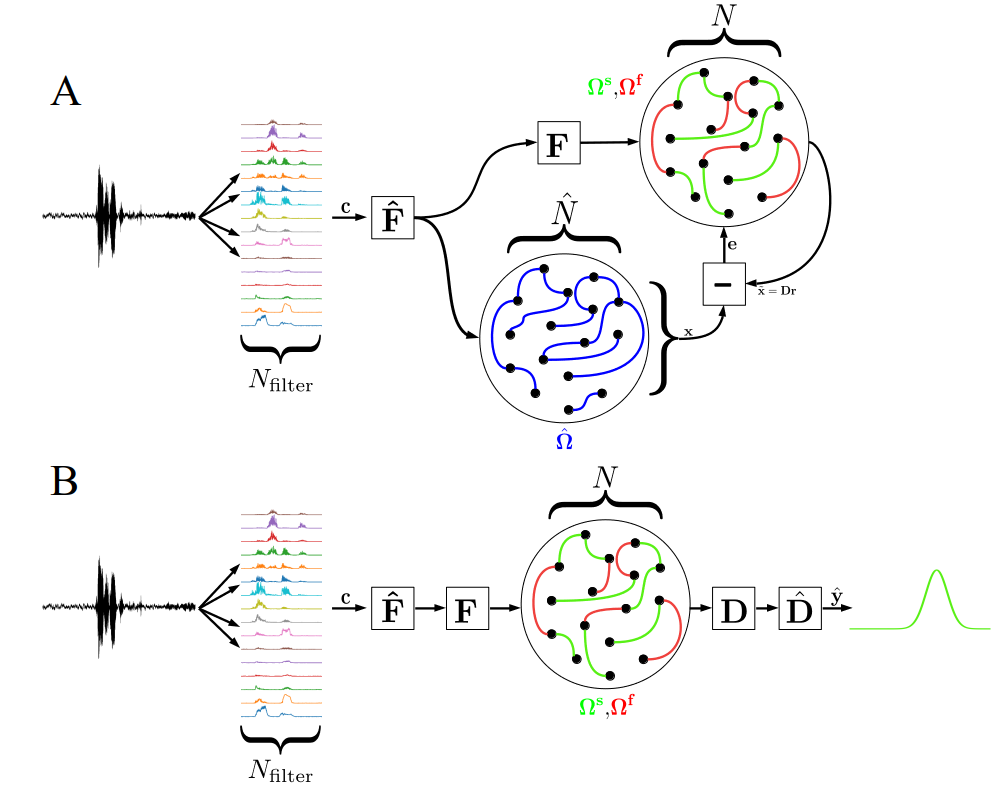
\includegraphics[width = \columnwidth, height=12cm]{figures/setup_complete.png}
  \caption{A high-level illustration of the training (\textbf{A}) and inference (\textbf{B}) process using the presented framework for an auditory classification task.
  \textbf{A:} During training, auditory samples are filtered using a set of band-pass filters with varying cut-off frequencies to produce a
  16 channel input, denoted $\mathbf{c}$. This input is then fed into the pre-trained rate network, which does inference on the presented signal. The dynamics
  $\mathbf{x}$ produced by the rate network are then used to compute the error $\mathbf{e} = \mathbf{x} - \hat{\mathbf{x}}$, which is then fed back into
  the spiking network using the feed-forward weights $\mathbf{D}^T$. Simultaneously, the spiking network receives the same input as the rate network, simply projected by the feed-forward
  weights $\mathbf{F} = \mathbf{D}^T$. Using the read-out weights $\mathbf{D}$, it then produces an estimation of the rate network dynamics $\hat{\mathbf{x}}$, which is then used to compute the
  error. \newline
  The inference mode, depicted in \textbf{B}, is straightforward: The now trained spiking network receives the same input the rate network would receive, but transformed using the
  feed-forward weights $\mathbf{F}$. It then produces the network dynamics $\tilde{\mathbf{x}} = \mathbf{D}r$ that closely match the ones of the rate network (if it would have received the signal)
  and produces the output $\tilde{\mathbf{y}} = \hat{\mathbf{D}}\tilde{\mathbf{x}}$. The value $\tilde{\mathbf{y}}$ is then thresholded to obtain the final prediction.}
  \label{fig:figure1}
\end{figure}

\section{Results}

\subsection{Temporal XOR}
In this experiment, a rate network of 25 neurons was trained to perform
temporal XOR on a one-dimensional input. The network was presented with two bumps
of magnitude $\pm 1$, indicating True or False. The bumps had a variable length
between 100 and 230ms and were separated by a 100ms pause, requiring the network
to memorize the first bump for some time. 

\begin{figure}[!htb]
  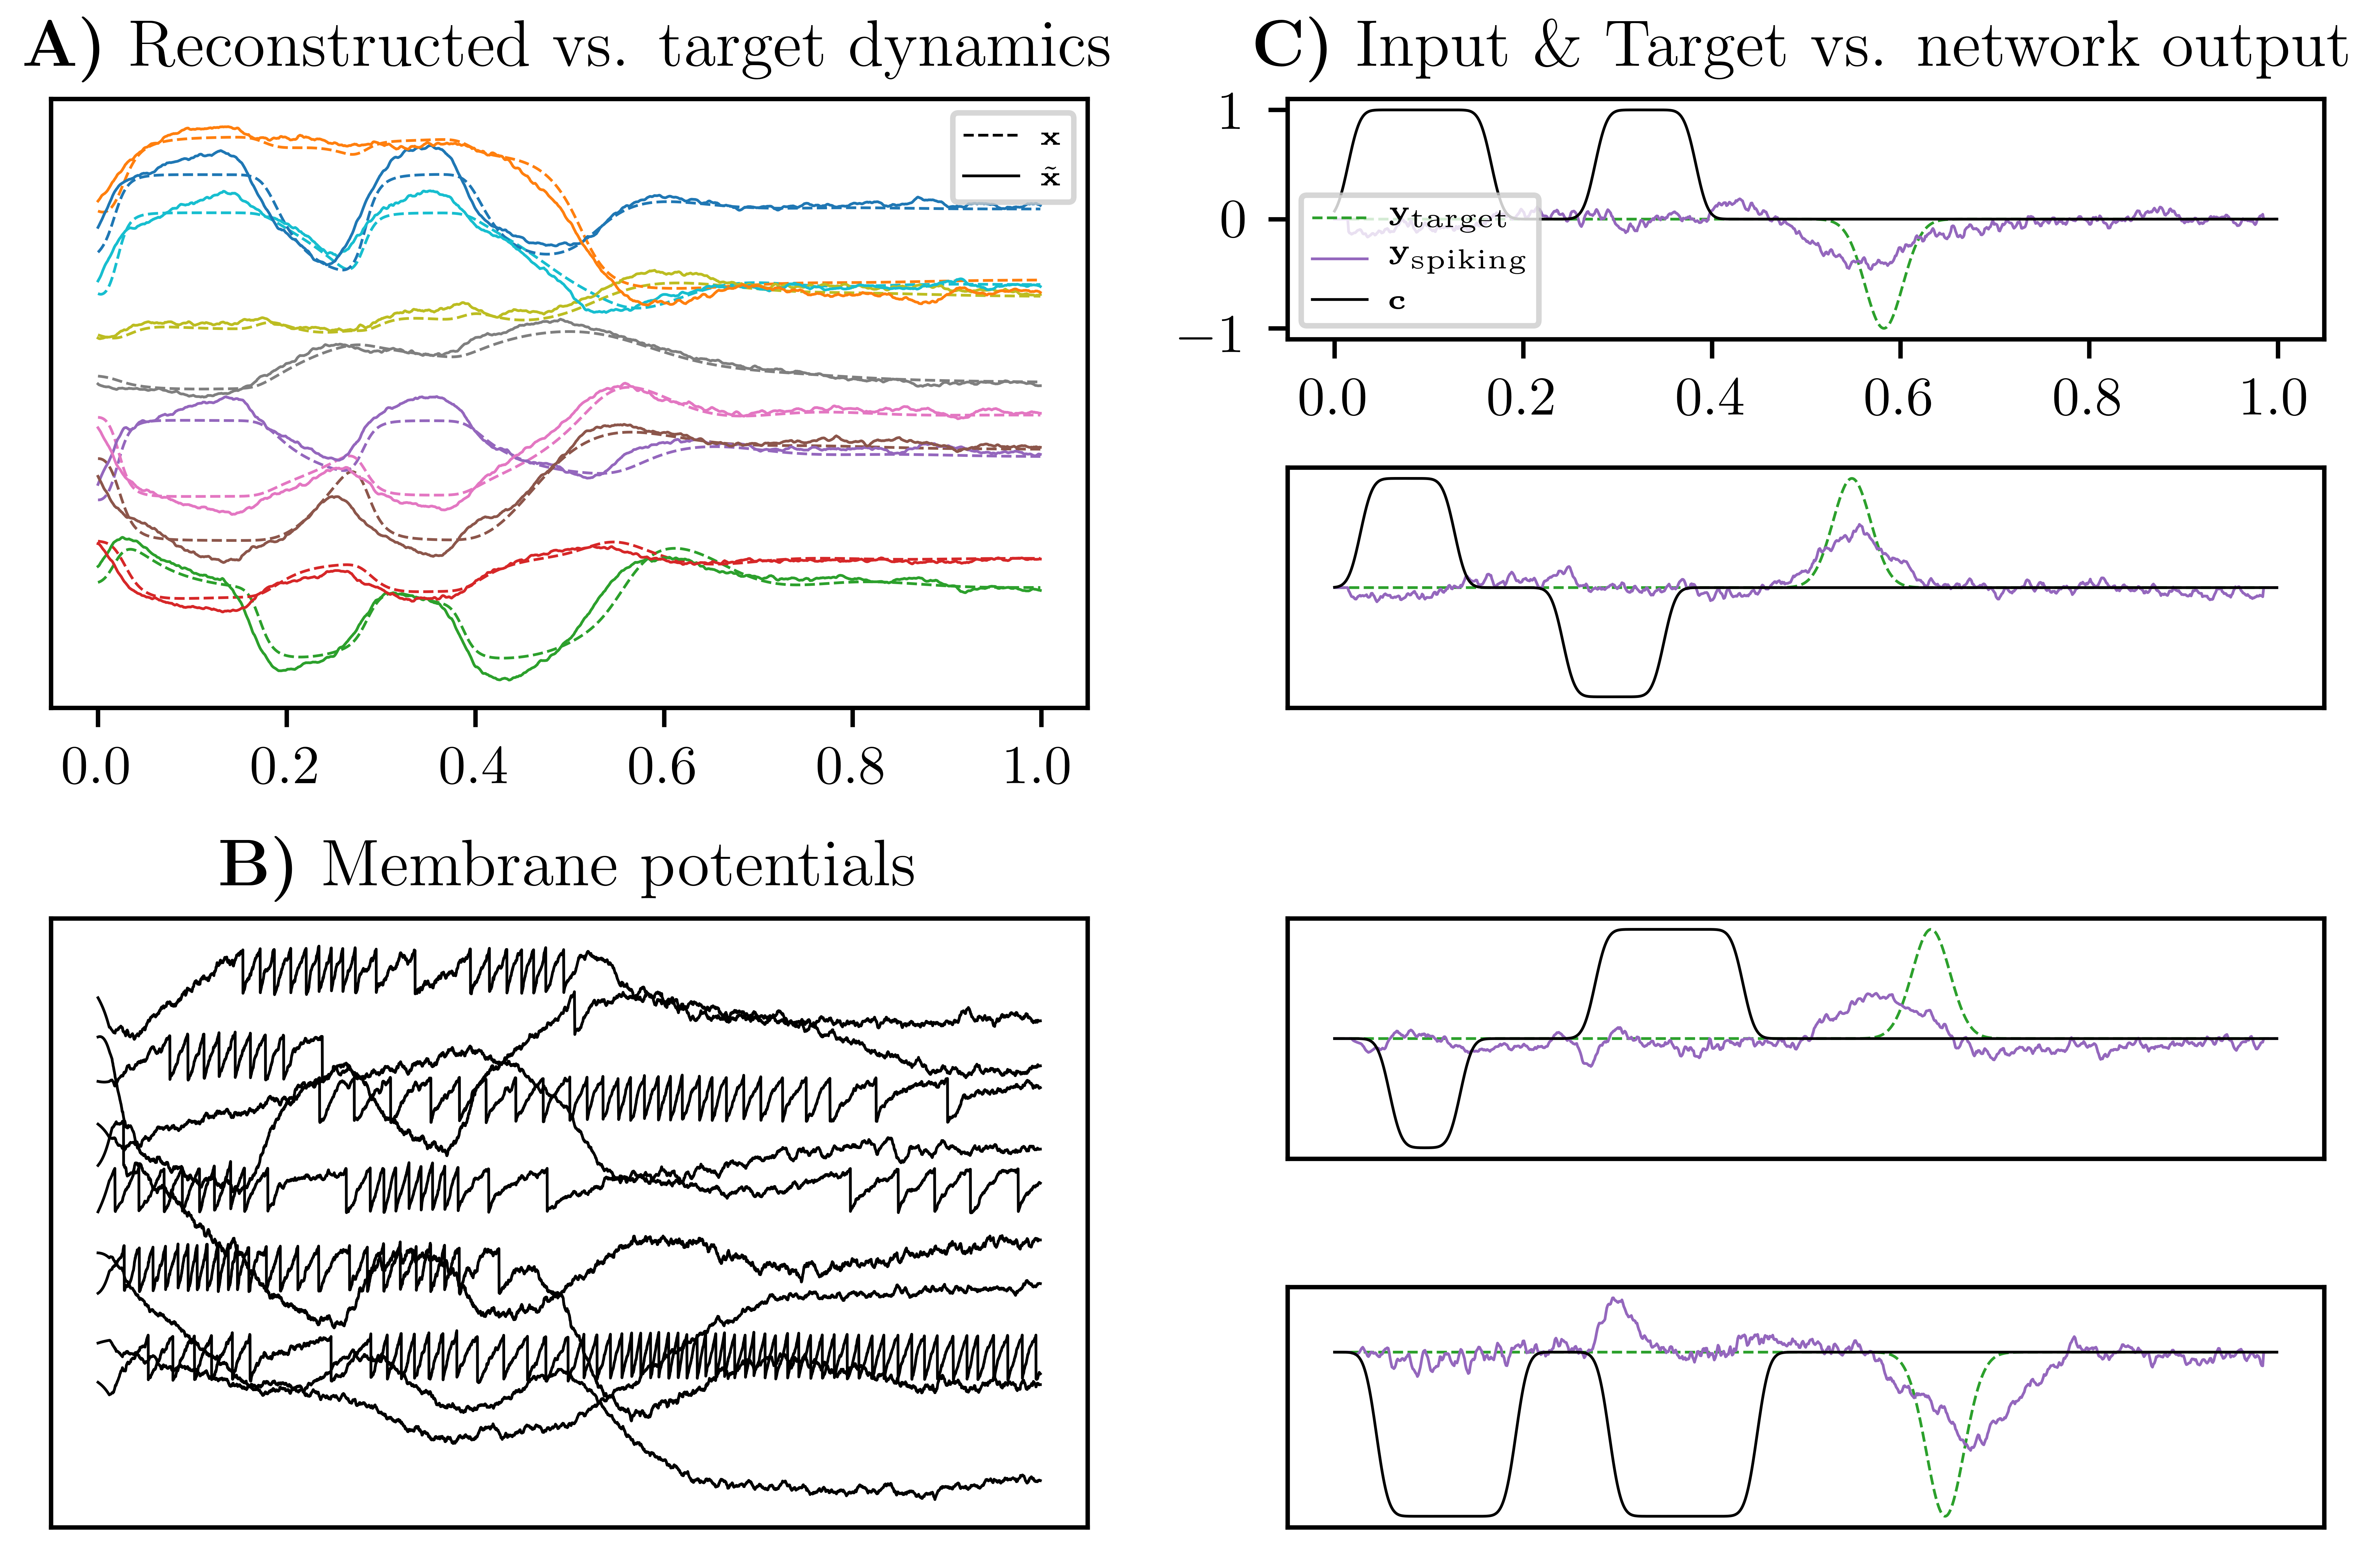
\includegraphics[width = \columnwidth, height=10cm]{figures/figure2.png}
  \caption{\textbf{A:} The spiking network consisting
  of 300 neurons successfully reconstructs the dynamics of the rate network.
  \textbf{B:} Due to the underlying balanced network, the membrane potentials show
  irregular and distributed spiking activity. [This is not the case yet, but should follow from the theory]
  \textbf{C:} Our network predicts 98\% of 300 unseen samples correctly. Note that although the
  reconstruction of the dynamics is quite precise, the later obatined response matches
  the target response quite poorly. This is simply due to the fact that a 25-dimensional
  rate network was the smallest possible rate network we could train to solve the task, meaning
  that every dimension of the dynamics is necessary to compute the final output to a high
  precision. To see that this is actually the reason, consider the second experiment:
  The reconstruction of the 128-dimensional dynamics is much worse compared to the temporal
  XOR task, but the final output still matches the actual target quite well.}
  \label{fig:figure2}
\end{figure}

\subsection{Wake-phrase detection}
To show that our approach also works on a more complex task, we used a network consisting of $N=1024$ spiking
neurons that learned to imitate a rate network with $\hat{N}=128$ units. The rate network was trained to recognize
a wake-phrase using roughly 10k training samples and 5k validation and testing samples. While the rate network
achieved a testing accuracy of ~90\%, our spiking imitator achieved ~85\% after training for only 10 epochs on about 500
training samples. We found that for training our network a learning rate schedule of the form $f(t)=a e^{(-t/b)}+c$
worked best, where $a=\eta_{initial}$, $c=\eta_\textnormal{end}$ and $b = (T/2) / \textnormal{ln}(100)$ with $T$ being the
total number of signal iterations. For the experiments conducted in this section, we chose $\eta_\textnormal{initial}=1e-4$ and $\eta_\textnormal{end}=1e-6$.
We also realized that having a schedule for the factor $k$ that controls the amount of error-feedback current is of high importance:
A constantly high $k$ results in no generalization during training since the network dynamics are governed by the error-feedback current and a too low
$k$ does not give the slow recurrent weights a chance to update correctly since the network is far from following the desired dynamics.
For these reasons, having a schedule for $k$ is extremely important. For this experiment, we chose a step function that decrements $k$ by a fixed amount
after some number of signal iterations. The reason we chose a step function is the following: 
If $k$ is constantly changing, even slowly, the amount of error-feedback current that "helps" the network
is constantly changing as well and does not give the slow recurrent weights a chance to adapt to the amount of "helper-current" that is
present in the network. We achieved best performance when we gave the slow recurrent weights some time to adapt to the current level by just
keeping $k$ constant for some time before decreasing it again.   

\begin{figure}[!htb]
  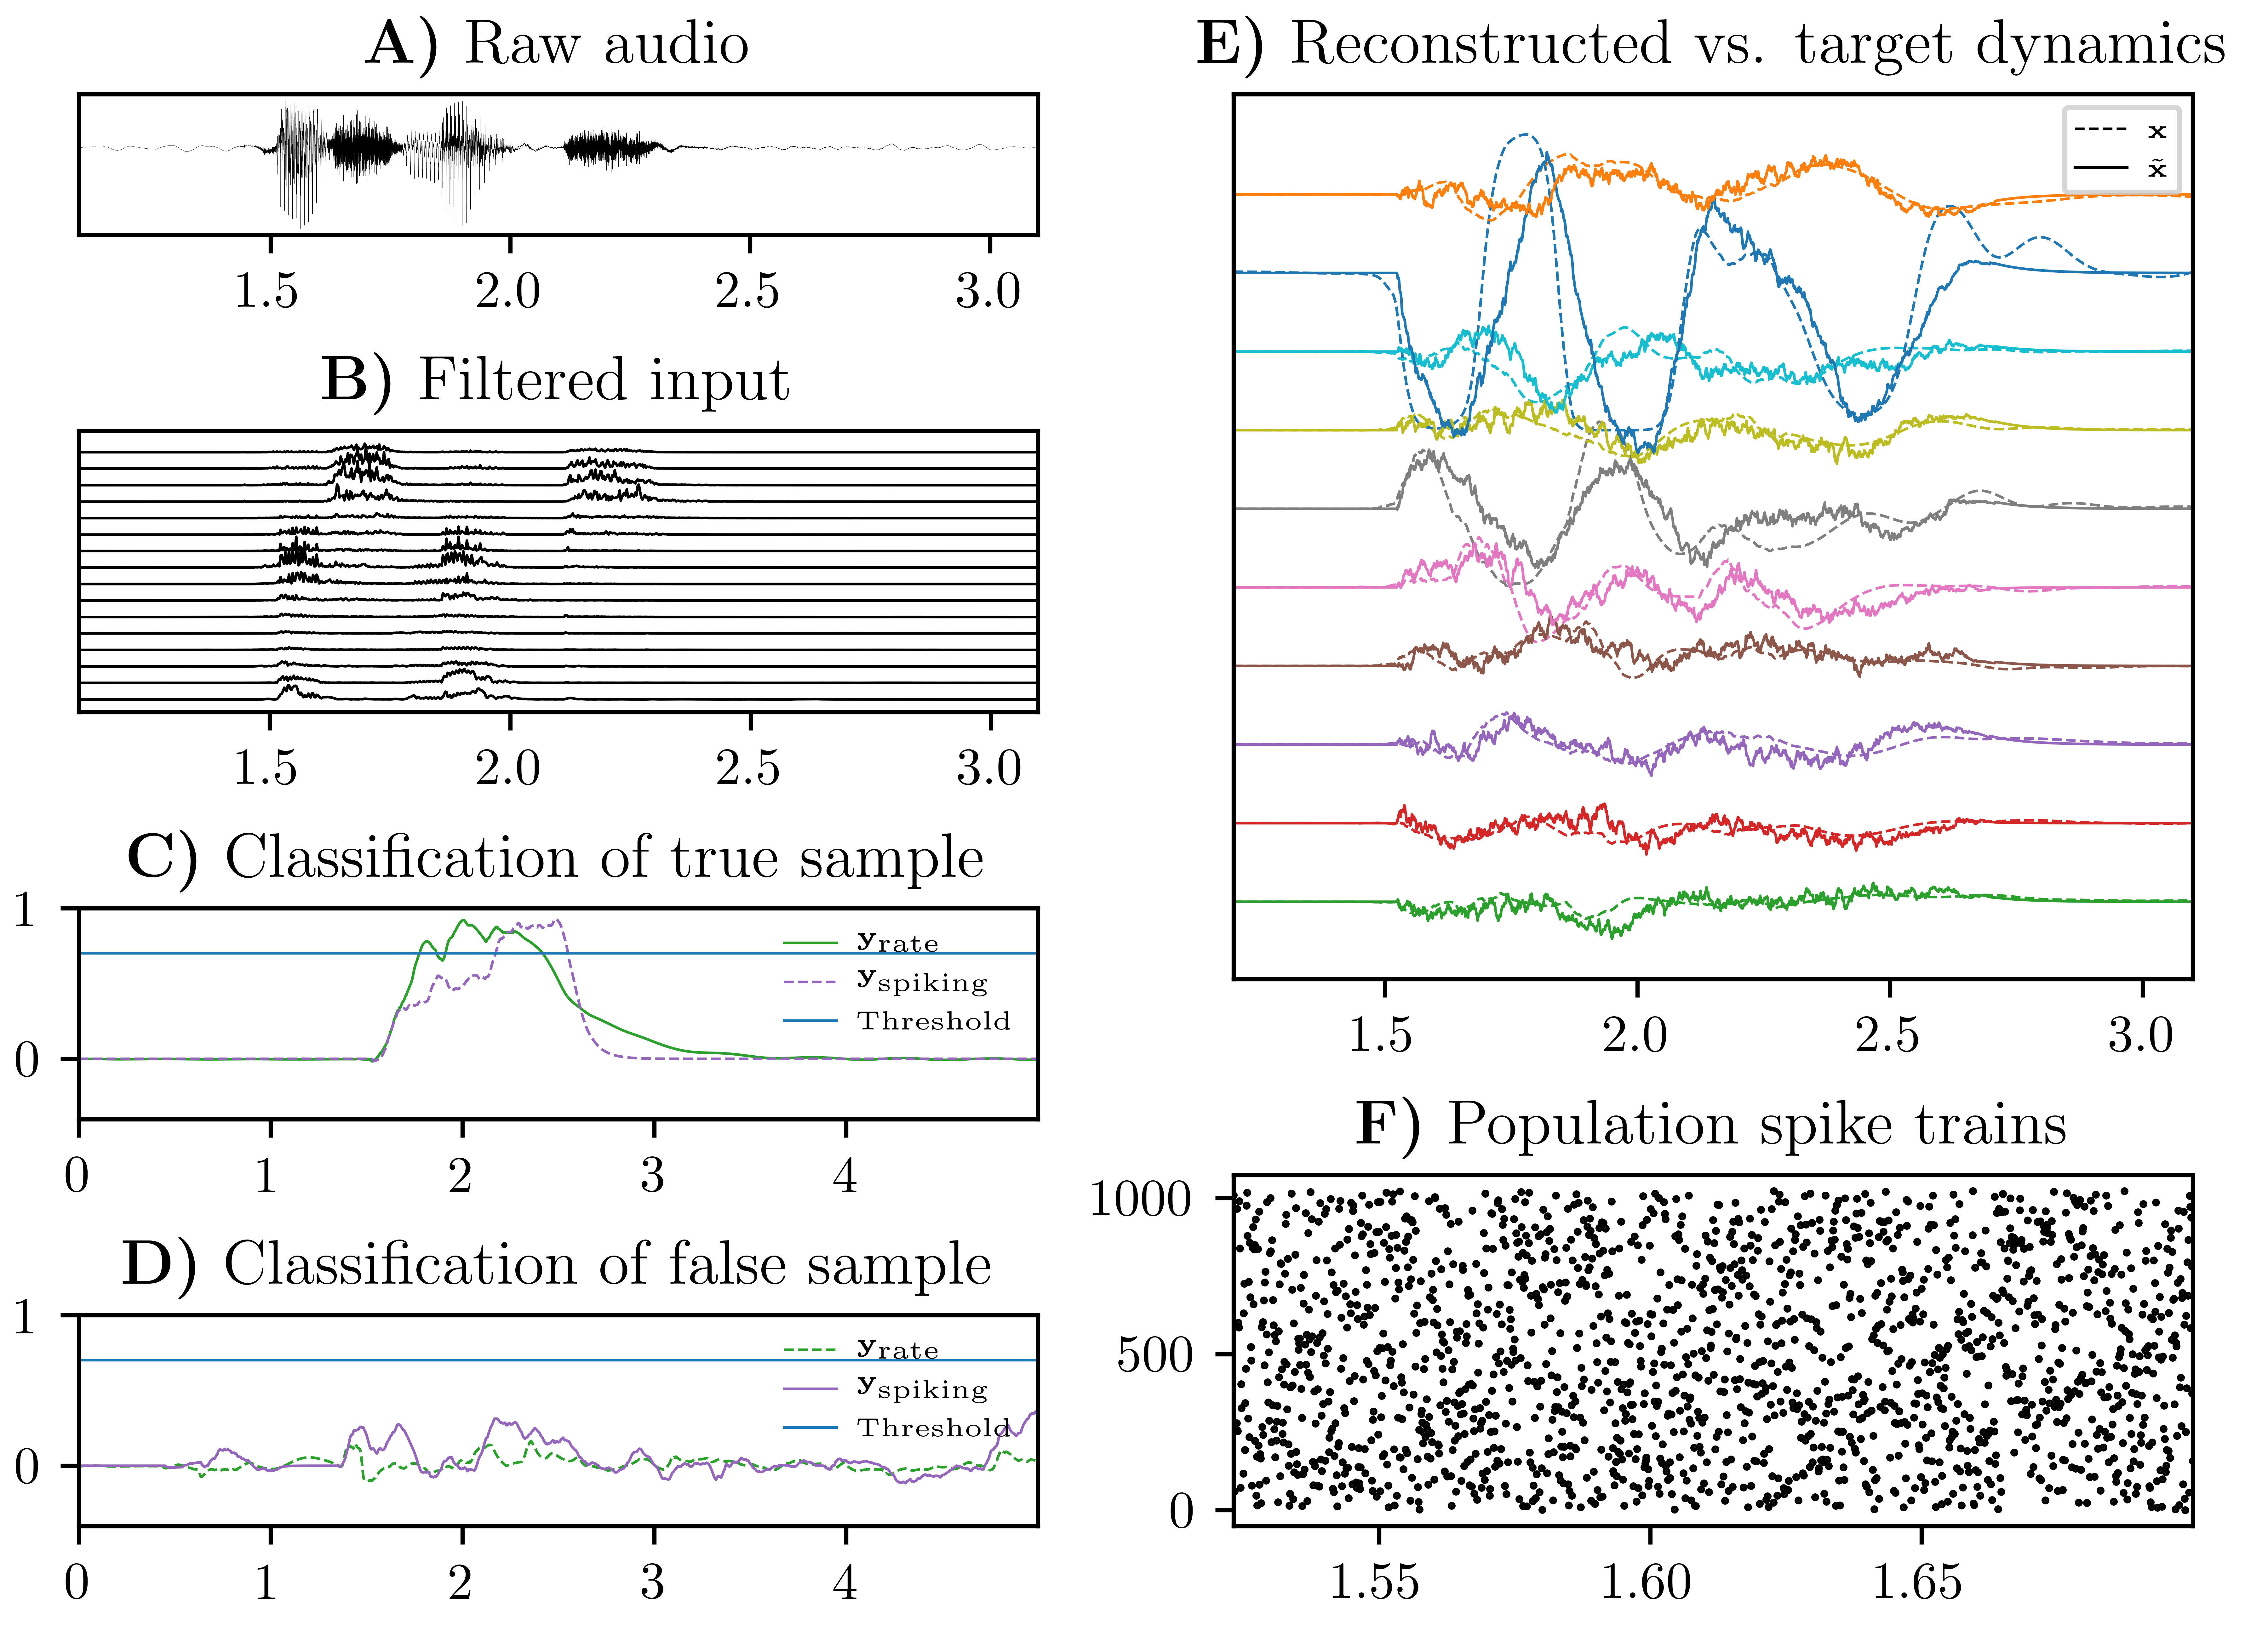
\includegraphics[width = \columnwidth, height=11cm]{figures/figure3.png}
  \caption{\textbf{A:} Audio samples either containing a key phrase, like "Wake up!", or plain talking were
  presented to the network, which then had to decide whether the input was the target phrase or not.
  \textbf{B:} To make classification easier, 16 butterworth filters with different cutoff frequencies
  were applied to create a 16-dimensional input signal. \textbf{C:} For a sample containing the key phrase,
  our network output closely follows the output of the rate network and thus makes the correct decision. In this experiment,
  a threshold at 0.6 determined whether the prediction was positive or negative. \textbf{D:} Negative samples on the other hand
  did not cause a rise in the output variable and were therefore correctly classified as negative samples. For this particular experiment,
  the rate network achieved 91\% on a held out test set containing 300 samples. The spiking network achieved 89.03\% test accuracy,
  while imitating the dynamics of the rate network (\textbf{E}). \textbf{F:} As expected, the spiking activity of the
  network is distributed and does not exhibit any output dependent patterns [This is not the case yet, but should follow from the theory].
  For this experiment, 2000 neurons were used, but a network of 1000 neurons achieves similar performance.}
  \label{fig:figure3}
\end{figure}

\subsection{Robustness}

On analog mixed-signal neuromorphic hardware components are not identical, which leads to a distribution
of parameters such as time constants or spiking thresholds. In this experiment, we simulated component mismatch by
distributing the synaptic- and membrane time-constants, as well as the spiking thresholds using a Gaussian distribution with mean
equal to the original value and the standard deviation being 20\% of the mean. Figure \ref{fig:figure5} demonstrates this behavior by plotting
the distributions of membrane time-constants on multiple cores on a neuromorphic processor, obtained through oscilloscope recordings.
Figure \ref{fig:figure4} shows the robustness of the network to component mismatch and sudden neuron failure for 300ms. Since neuromorphic
processors, analog or digital, are furthermore constrained in the resolution of their weights, which also can be seen as a type of noise,
we reduced the total weights to 3 and 4 bit floating point values. To integrate the low-resolution weights into training, we kept a
full-precision version of the weights and adapted them using the updates computed from the low-resolution network. Not surprisingly,
this method yields much better results than just reducing the precision of the weights post-learning. Table \ref{table:table1} shows the
testing accuracies for 1000 samples using the networks perturbed by various noise sources.

\begin{figure}[!htb]
  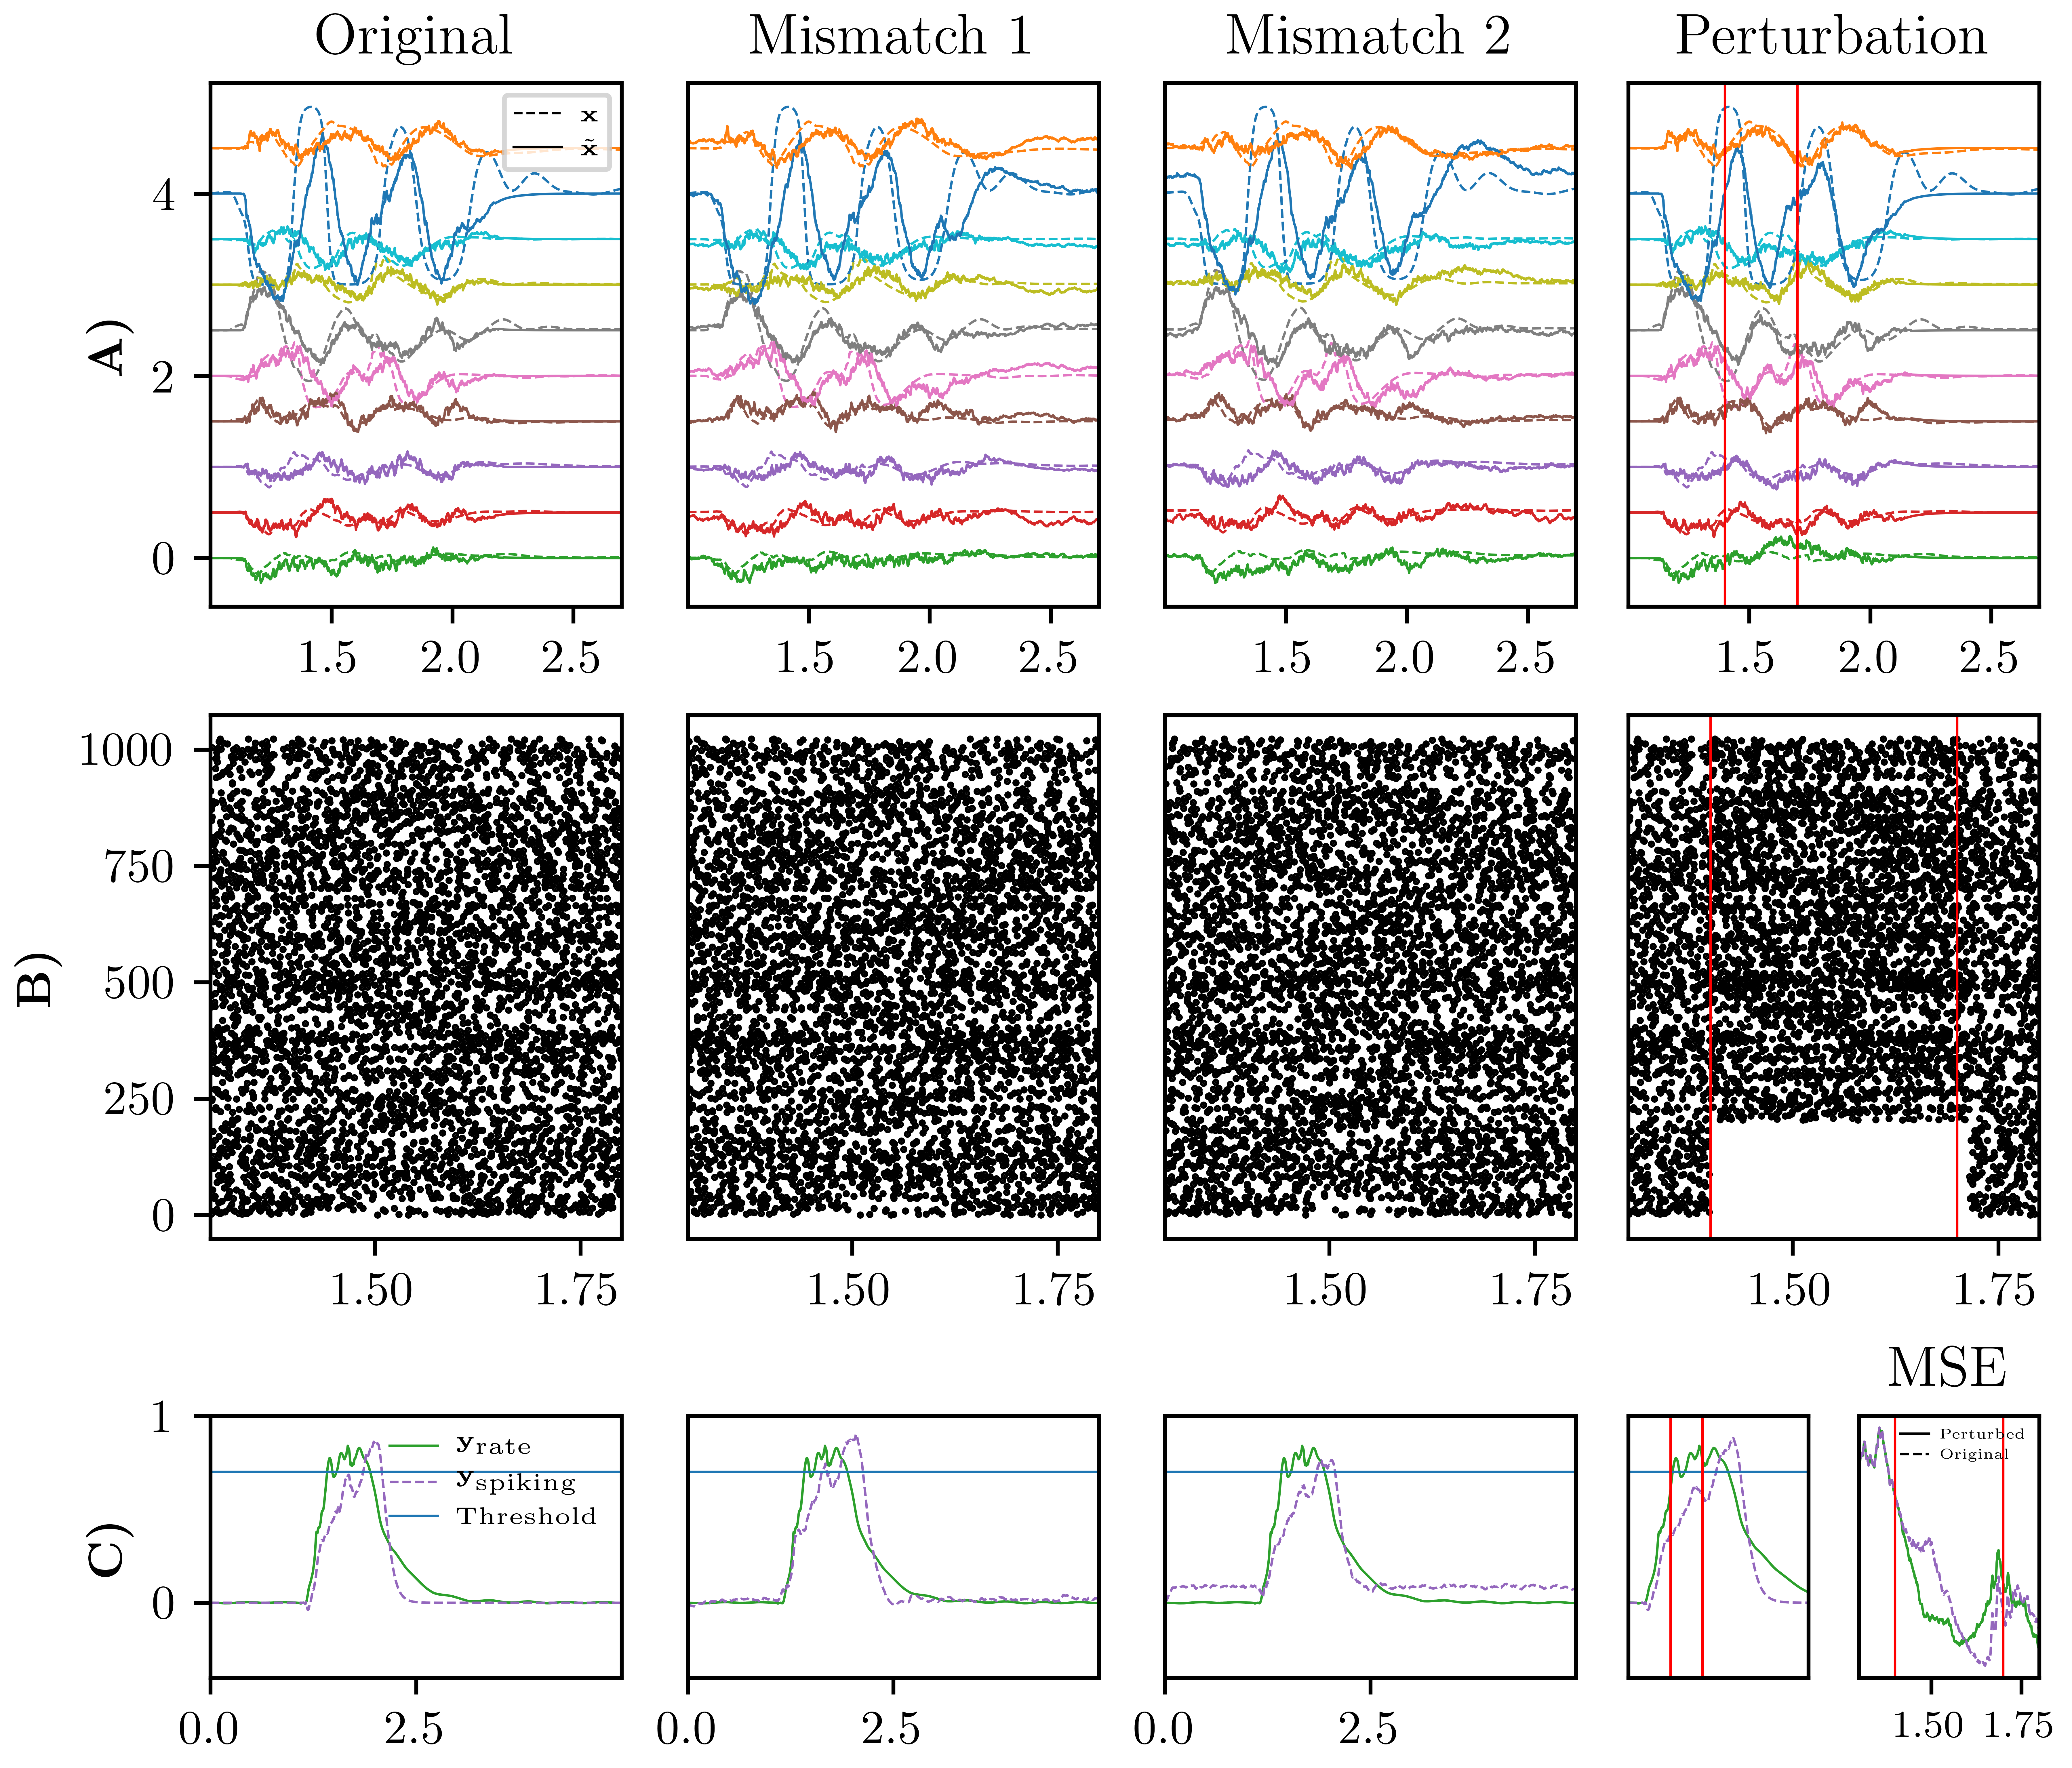
\includegraphics[width = \columnwidth, height=13cm]{figures/figure4.png}
  \caption{\textbf{A:} Reconstruction of the 128-dimensional target dynamics (only first 10 dimensions are shown). \textbf{B:} Here,
  one can observe the effect of the mismatch on the recurrent dynamics. Due to the distribution of the neuron- and synaptic
  time-constants, recurrent activity is sustained a little longer with some individual neurons spiking at a higher frequency.
  In the last network instance, we clamped 20\% of the neurons at a crucial time during classification. However, as can be seen
  in \textbf{C}, the reconstruction is stable, as well as the final output. It should also be noted that
  for 20\% clamped neurons, the mean-squared error (MSE) did not increase during the time the neurons were shut off.}
  \label{fig:figure4}
\end{figure}

\begin{table}[!htb]
  \begin{adjustbox}{center} \label{table:table1}
  \begin{tabular}{|l|l|l|l|l|l|}
  \hline
  {Original} & {Mismatch I} & {Mismatch II} & {Quantised to 4 bits} & {Quantised to 3 bits} & {Rate network} \\
  \hline
  {85.31\%}  & {79.20\%}    & {85.91\%}     & {84.02\%}             & {84.02\%}             & {90.51\%}      \\
  {84.62\%}  & {83.91\%}    & {85.11\%}     & {84.32\%}             & {84.32\%}             & {89.11\%}      \\
  {83.33\%}  & {84.42\%}    & {86.21\%}     & {83.12\%}             & {83.12\%}             & {91.21\%}      \\
  {84.92\%}  & {83.91\%}    & {85.11\%}     & {83.22\%}             & {83.22\%}             & {89.91\%}      \\
  \hline
  \end{tabular}
\end{adjustbox}
\caption{Test accuracies over 5 trials on 1000 samples for networks perturbed by different kinds of noise. [NEEDS FIXING]}
\end{table}

\begin{figure}[!htb]
  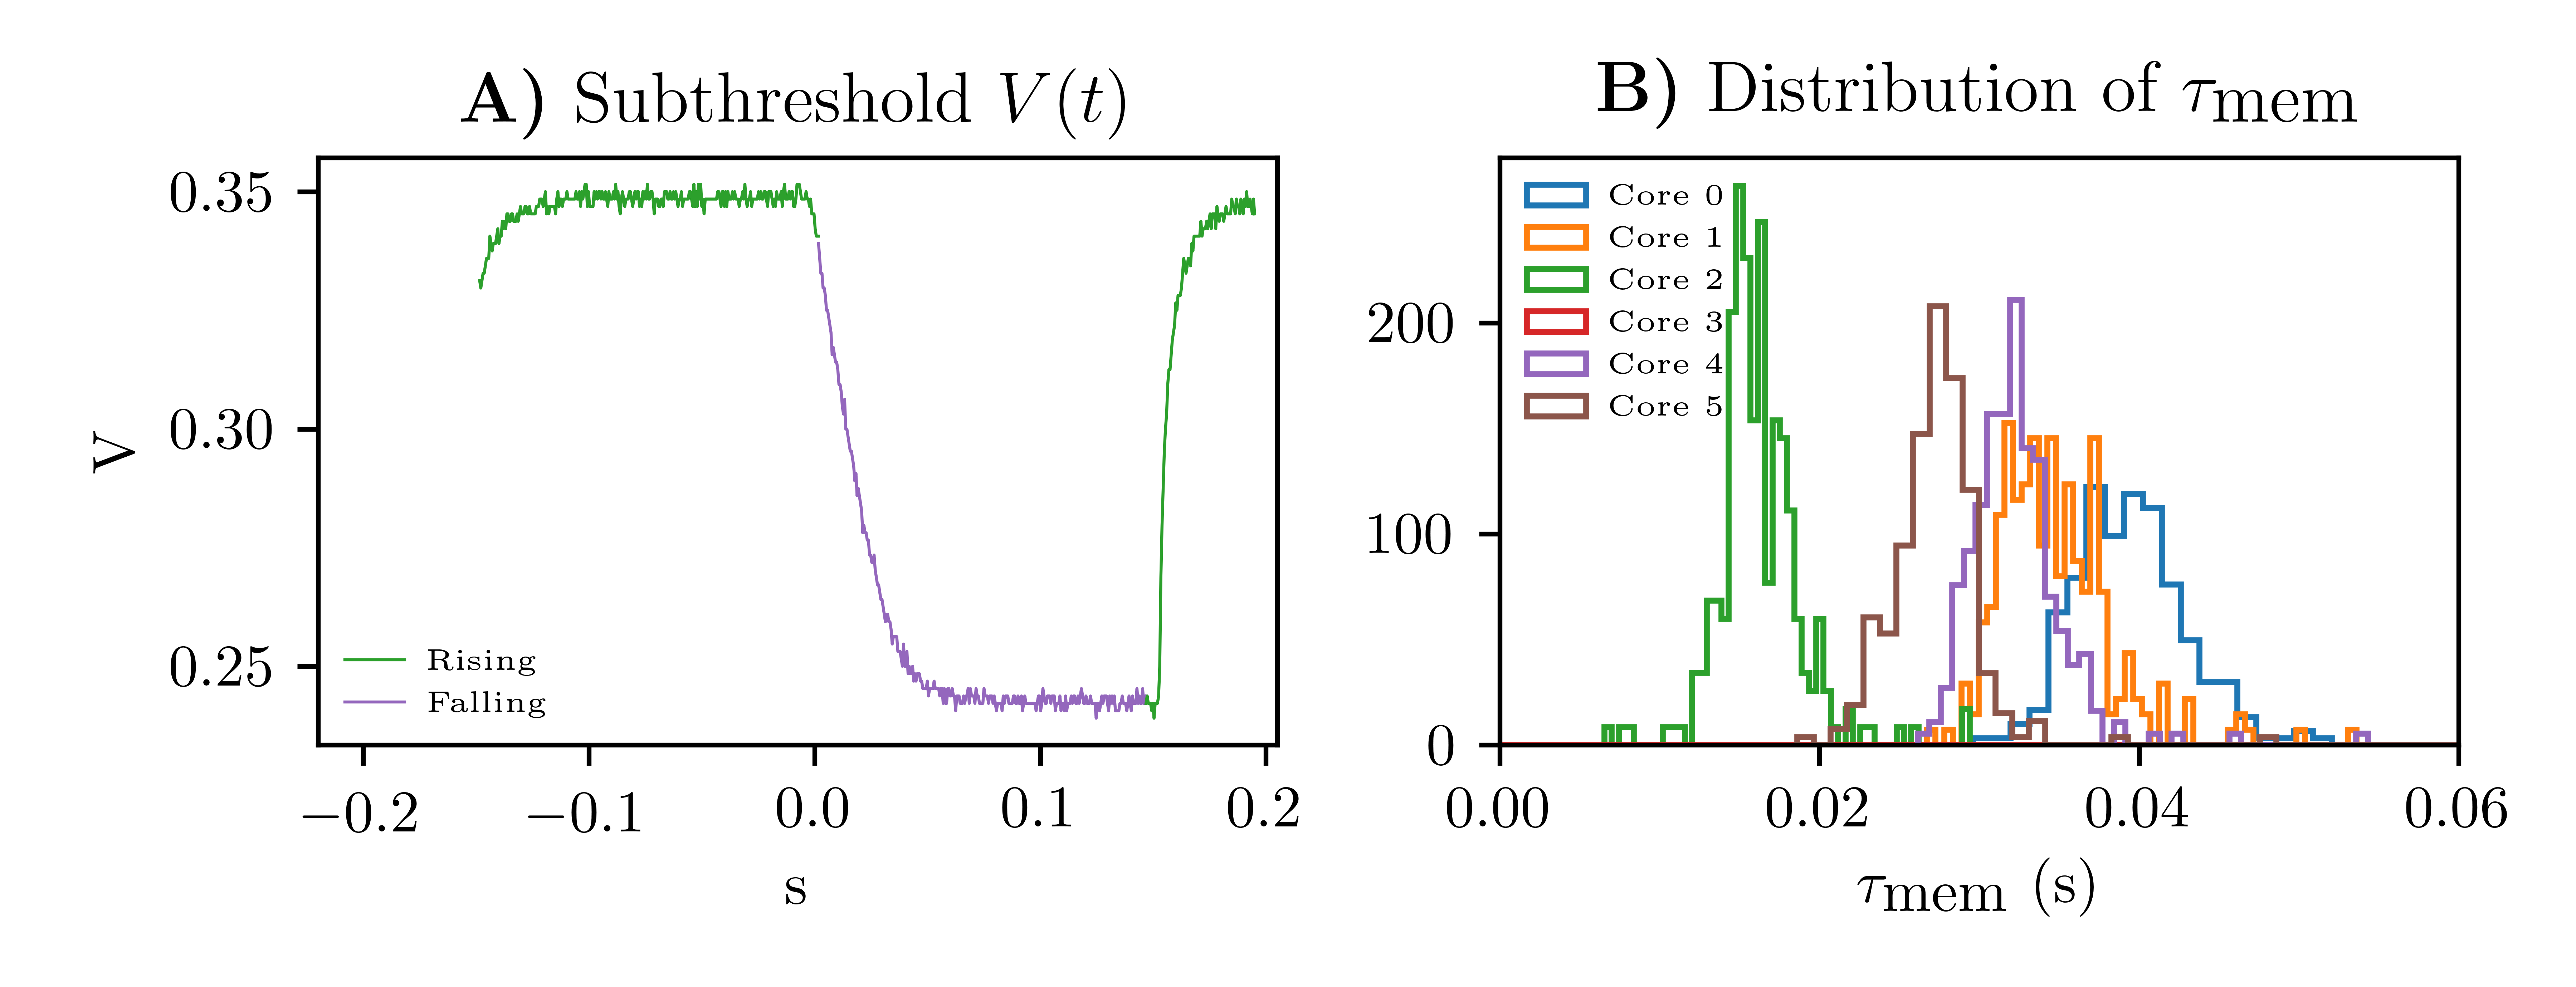
\includegraphics[width = \columnwidth, height=6cm]{figures/figure5.png}
  \caption{\textbf{A} shows an example of such a recording. \textbf{B:} The membrane time-constants of neurons for different expected time-constants.
  It can be seen that as the time constant increases, also the standard deviation increases (thus $\sigma=0.2\mu$).
  The time-constants were computed by fitting an exponential to subthreshold recordings of each neuron.}
  \label{fig:figure5}
\end{figure}

[INTERESTING: FAST CONNS GOOD FOR NEURON LOSS?]

\clearpage

\vskip 0.2in
\bibliography{bibliography}

\end{document}